\section{Product perspective}
The basic idea upon which the system will be built is that the user is a volounteer, so it has to put as little effort as possible to send information about violations.

Right after the user enters the application, it can take a picture directly from there. Then the taken picture is scanned by an OCR algorithm that detects (or at least tries to) the biggest licence plate and obtains its number. The application proceeds to collect as much data as possible from the built-in functions of the host device: gets the time, date and retrieves location through GPS. The auto-collected data is then showed to the user who can correct or complete it.
Finally the user inserts the infraction type and the violation is ready to be sent to the authorities. At this point the violation is still linked to the user which makes it, but as soon as the violation is sent to the authorities, it becomes anonymous. This difference can be clearly seen in Figure \ref{fig:classDiagram} below. We have two subclasses of the superclass \emph{Violation}: \emph{UserEndViolation} and \emph{AuthorityEndViolation}. The latter is anonymous and is enriched with two states: accepted/discarded and the level of priority.

% Insert class diagram
\begin{figure}[H]
    \centering
    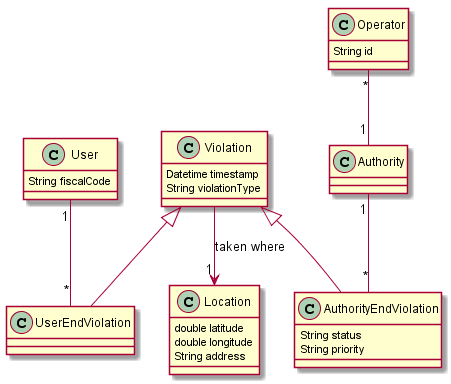
\includegraphics[width=0.5\linewidth]{../diagrams/classDiagram.png}
    \caption{Class diagram}
    \label{fig:classDiagram}
\end{figure}

Figure \ref{fig:violationDiagram} shows the evolution of a Violation, from when the user takes the picture, to the final user review.

% Insert state_diagram_violation
\begin{figure}[H]
    \centering
    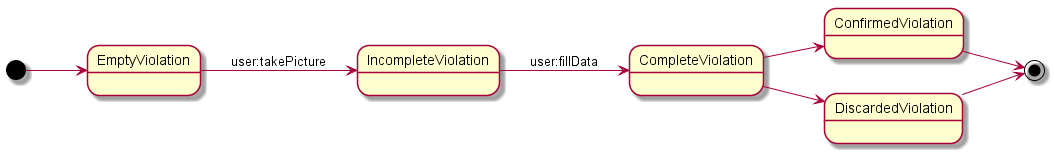
\includegraphics[width=\linewidth]{../diagrams/state_diagram_violation.png}
    \caption{Violation state diagram}
    \label{fig:violationDiagram}
\end{figure}

Notice that depending on the quality of the picture taken, the OCR algorithm may fail, in this case the user is asked to take another, possibly better, picture. 

Figure \ref{fig:acceptViolationDiagram} shows what happens when an operator takes care of a Violation that is received by the authority. As explained before, firstly it has to accept or discard the violation, then in case of acceptance assign it a level of priority so that another department can better schedule the intervention

% Insert state_diagram_accept_violation
\begin{figure}[H]
    \centering
    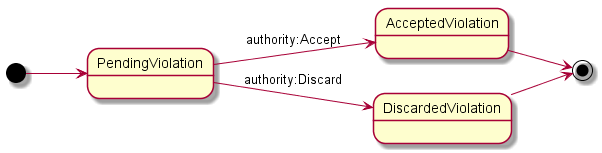
\includegraphics[width=\linewidth]{../diagrams/state_diagram_accept_violation.png}
    \caption{Accept Violation state diagram}
    \label{fig:acceptViolationDiagram}
\end{figure}